%
% teil1.tex -- Beispiel-File für das Paper
%
% (c) 2020 Prof Dr Andreas Müller, Hochschule Rapperswil
%
%
% teil2.tex -- Beispiel-File für teil2 
%
% (c) 2020 Prof Dr Andreas Müller, Hochschule Rapperswil
%%



\rhead{Kalman-Filter}

\section{Kalman-Filter}
Die interessante Grösse ist also das Integral der Überlagerung zweier Kräfte. 
Wir brauchen also die zweite Ableitung der Messung, ohne deren Eigendynamik.
Da wir die äussere Kraft nicht direkt messen können, benötigen wir ein Werkzeug, welches aus der gemessenen Position, die Krafteinwirkung auf unsere System schätzt. 
Dies ist eine typische Anwendung für das Kalman-Filter.

Das Filter schätzt den Zustand eines Systems anhand von Messungen und kann den nächsten Zustand errechnen und aus dieser Schätzung auch eine erwartete Messung herleiten.
Das Filter berücksichtigt dazu nicht nur die Messung und den Zustand, sondern auch die Unsicherheiten dieser beiden Grössen, welche als Parameter in das Modell des Systems einfliessen.

Unser Ziel ist es, anhand der Messung die eigentlich interessante Grösse $f$ zu bestimmen. 
Durch Kenntnis über den aktuellen Zustand und der Eigendynamik des Systems berechnen wir eine Vorhersage des nächsten Zustandes.
Die für das Filter relevante Grösse ist dann nicht mehr die eigentliche Messung, sondern die Differenz aus Messung und Vorhersage, da diese Differenz, die Innovation, eine Aussage über die nicht-deterministischen, externen Einflüsse auf das System ermöglicht.

Die genau Herleitung des Kalman-Filter befindet sich für Interessierte im Wahrscheinlichkeit und Statistik Skript von A. Müller. 
Im folgenden Abschnitt werden die Resultate zitiert. 

\subsection{Geschichte}
Das Kalman-Filter wurde 1960 von Rudolf Emil Kalman entdeckt und direkt von der NASA für die Appollo Mission benutzt.
Das Filter kommt mit wenig Rechenleistung aus und war somit dafür geeignet die Rakete bei der Navigation zu unterstützen. 
Eine typische Anwendungen des Kalman-Filters ist Glättung von verrauschten Daten und die Schätzung von Parametern. Dies kommt heutzutage in jedem Satellit, Navigationssystem, Smartphones und Videospielen vor.

\subsection{Exkurs Wahrscheinlichkeit} 
	\label{erdbeben:Wahrscheindlichkeit} 
Das Kalman-Filter schätzt den wahrscheinlichsten Wert zwischen Normalverteilungen, in unserem Fall sind dies die Messung und die Vorhersage.
Dies bedeutet, das Filter schätzt nicht nur den Mittelwert, sondern auch die Standartabweichung.
Da Normalverteilungen dadurch vollständig definiert sind, schätzt ein Kalman-Filter die gesamte Verteilungsfunktion des Zustandes.
In der Abbildung~\ref{erdbeben:Gauss3} sind zwei Funktionen dargestellt. 
Die eine Funktion zeigt die errechnete Vorhersage des Zustands, bzw. deren Normalverteilung. 
Die andere Funktion zeigt die verrauschte Messung des nächsten Zustand, bzw. deren Normalverteilung. 
Wie man am Beispiel der Gauss-Verteilungen in Abblidung~\ref{erdbeben:Gauss3} sehen kann, ist sowohl der geschätzte Zustand als auch der gemessene Zustand normalverteilt und haben dementsprechend unterschiedliche Standardabweichungen $\sigma$ und Erwartungswerte $\mu$. Das folgende wird in~\cite{erdbeben:aragher_understanding_2012}beschrieben.

Wir haben eine Vorhersage aus der Systemdynamik und eine Messung des Zustandes.
Diese widersprechen sich im Allgemeinen. 
Jedoch wissen wir die Wahrscheinlichkeiten der beiden Aussagen. 
Um eine genauere Schätzung des Zustandes zu machen, wird nun ein Wert zwischen den beiden Verteilungen berechnet. 
Nun wird eine Eigenschaft der Normalverteilung ausgenutzt. Durch das Multiplizieren zweier Normalverteilungen entsteht eine neue Normalverteilung. 
Wir haben eine Normalverteilung der Vorhersage:
\[ 
{y_1}(x;{\mu_1},{\sigma_1})=\frac{1}{\sqrt{2\pi\sigma_1^2}}\quad e^{-\frac{(x-{\mu_1})^2}{2{\sigma_1}^2}} 
\]
und der Messung:
\[ 
{y_2}(x;{\mu_2},{\sigma_2})=\frac{1}{\sqrt{2\pi\sigma_2^2}}\quad e^{-\frac{(x-{\mu_2})^2}{2{\sigma_2}^2}}.
\]
Diesen werden nun multipliziert und durch deren Fläche geteilt um sie wieder zu normieren, $\odot$ beschreibt dabei die Multiplikation und die Normierung auf den Flächeninhalt eins :
\begin{align*}
	{y_f}(x; {\mu_f}, {\sigma_f}) 
	&=
	 {y_1}(x;{ \mu_1},{ \sigma_1}) \odot {y_2}(x; {\mu_2}, {\sigma_2})
	\\
	&=
	\frac{1}{\sqrt{2\pi\sigma_1^2}}\quad e^{-\frac{(x-{\mu_1})^2}{2{\sigma_1}^2}} \odot \frac{1}{\sqrt{2\pi\sigma_2^2}}\quad e^{-\frac{(x-{\mu_2})^2}{2{\sigma_2}^2}}
	\\
	&=
	\frac{ \frac{1}{\sqrt{2\pi\sigma_1^2}}e^{-\frac{(x-{\mu_1})^2}{2{\sigma_1}^2}} \cdot \frac{1}{\sqrt{2\pi\sigma_2^2}}e^{-\frac{(x-{\mu_2})^2}{2{\sigma_2}^2}}}{\int {y_1} {y_2} dx}.
\end{align*}
Durch geschicktes umformen resultiert aus der Kombination der beiden Verteilungen wiederum in einer Normalverteilung
mit Erwartungswert
\[ \mu_f = \frac{\mu_1\sigma_2^2 + \mu_2 \sigma_1^2}{\sigma_1^2 + \sigma_2^2} \]
und Varianz
\[
\sigma_f^2 = \frac{\sigma_1^2 \sigma_2^2}{\sigma_1^2 + \sigma_2^2}.
\]
Dadurch gleicht sich die neue Kurve den anderen an. Interessant daran ist, dass die fusionierte Kurve sich der genauere Normal-Verteilung anpasst.
Ist ${\sigma_2}$ klein und ${\sigma_1}$ gross, so wird sich die fusionierte Kurve näher an ${y_2}(x;{\mu_2},{\sigma_2})$ begeben.
Somit ist $\mu_f$ das gewichtete Mittel der beiden $\mu_{1,2}$ und die Varianzen sind die Gewichte. 
Das Interessante an $\mu_{f}$ ist, dass ${\mu_2}$  ${\sigma_1}$ beeinflusst. 
Somit beeinflusst die Messung die Schätzung und umgekehrt.
Die neue Funktion ist die best mögliche Schätzung für zwei Verteilungen, welche den selben Zustand beschreiben. 
Dies ist in der Abbildung~\ref{erdbeben:Gauss3} anhand der rote Funktion ersichtlich. 
\begin{figure}
 \begin{center}
 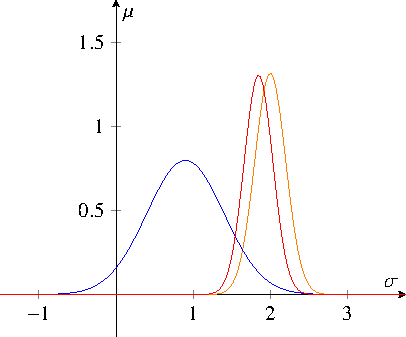
\includegraphics[width=5cm]{papers/erdbeben/Gausskurve3.pdf}
 \caption{Durch das Multiplizieren der blauen Mess- und der orangen Schätz-Verteilung entsteht die die rote, optimale Funktion}
 \label{erdbeben:Gauss3}
 \end{center}
\end{figure}

Was in zwei Dimensionen erklärt wurde, funktioniert auch in mehreren Dimensionen. 
Dieses Prinzip mach sich das Kalman Filter zu nutze, und wird von uns für die Erdbeben Berechnung genutzt. 

\subsection{Filter-Matrizen}
Da wir nun ein Werkzeug besitzen, dass die Beschleunigung, welche auf das Gehäuse wirkt, ermitteln kann, wird dieses nun Schritt für Schritt erklärt. 
Um den Kalman Filter zu starten, müssen gewisse Bedingungen definiert werden. 
In diesem Abschnitt werden die einzelnen Parameter und Matrizen erklärt und erläutert, wofür sie nützlich sind. 

Dabei muss genau auf den Index geachtet werden. Nach dem Artikel~\cite{erdbeben:wikipedia} ist die Indexierung so genormt:
Der Zeitschritt wird mit $k$ definiert, $k-1$ ist somit ein Zeitschritt vor $k$.
Auf der linken Seite von | wird der aktuelle Zustand verlangt, bzw. ausgegeben, auf der rechten Seiten den bisherigen Zustand.
Dies bedeutet, dass die Notation $x_{n|m}$ die Schätzung von $x$ zum Zeitpunkt $n$ bis und mit zur Zeitpunkt $m \leq \ n$ präsentiert. 

\subsubsection*{Vorhersage}
Im Filterschritt Vorhersage wird der nächste Zustand anhand des Anfangszustand und der Systemmatrix berechnet. 
Die Systemmatrix $A$ beschreibt ein kontinuierliches System $\dot x = Ax$. 
Wir benötigen jedoch ein Zeit-diskretes System $x_{k+1} = \Phi x_k$.
Die Exponentialfunktion $\exp(At)$ beschreibt die Entwicklung eine Zustandes im Laufe der Zeit.
Die Übergangs-Matrix $\Phi$ erhalten wir folglich aus der Systemdynamikmatrix mittels Exponentialfunktion: 
\[\Phi = \exp(A\Delta t). \]
Die Matrix $\Phi$ beschreibt die Übergänge zwischen zeitlich aufeinanderfolgenden Zuständen $x_{k-1}$ und $x_{k}$ anhand folgender Gleichung:
\[
{x_{k|k-1}}=\Phi{x_{k-1|k-1}}= \exp(A\Delta t){x_{k-1|k-1}}.
\] 

Im Abschnitt ~\ref{erdbeben:Wahrscheindlichkeit} benötigten wir die Varianzen der Normalverteilungen. 
Im mehrdimensionalen Fall übernimmt dies die Kovarinanzmatrix $P$.
Sie wird in jedem Schritt aktualisiert. 
Dazu wird noch die Prozessunsicherheit $Q$ addiert, somit entsteht die Gleichung
\[
{P_{k|k-1}}=\Phi {P_{k-1|k-1}} {\Phi _{k}}^T + {Q_{k-1}}.
\] 
Es vergeht genau $\Delta t$ Zeit, und dieser Vorgang wird wiederholt.  
Das Filter passt sich selber an und korrigiert sich bei grosser Abweichung.

\subsubsection*{Messen}
Der Sensor wurde noch nicht benutz, doch genau der liefert Werte für das Filter. 
Aus der Vorhersage des Zustandes $x_{k|k-1}$ und der Messmatrix $H$ erhalten wird eine Vorhersage der Messung. 
Die Innovation
\[
{w_{k}}={z_{k}}-{H}{x_{k|k-1}}
\] 
beschreibt, wie genau die Vorhersage den aktuellen Messwert $z$ mittels der Systemmatrix $\Phi$ beschreiben kann. 
Die Innovation ist der Teil der Messung, der nicht im Modell erfasst ist.
Dies leuchtet ein, eine Innovation von $0$ bedeutet, dass die Messung nichts Neues hervorbrachte.
Für eine schlechte Vorhersage wird die dazugehörige Innovation gross, für eine genaue Vorhersage dagegen klein sein. 
Entsprechende Korrekturen werden dann gross bzw. nur gering ausfallen. 

\subsubsection*{Aktualisieren}

Für eine optimale Schätzung des Zustandes muss die Vorhersage entsprechend der Innovation korrigiert werden.
In der Literatur findet man für eine optimales Korrektur die Gleichungen:
\begin{align*}
{S_{k}} &={H}{P_{k|k-1}}{H}^T+{R_{k}}
\\
{K_{k}} &= {P_{k|k-1}} {H^T}{S_{k}^{-1}}
\end{align*}
Dabei ist $K$ das Kalman-Gain. 
Mit dessen Hilfe erhalten wir die optimale Schätzung des nächsten Zustandes
\[
{x_{k|k}}={x_{k|k-1}}+{K_{k}}{w_{k}}.
\] 
Dazu kommt eine neue Kovarianz $P$ für den nächste Vorhersageschritt:
\[
{P_{k|k}}=(I-{K_{k}}{H}){P_{k|k-1}} 
\] 
Der ganze Algorithmus ist nun vollständig und beginnt wieder mit der Vorhersage 
\[
{x_{k|k-1}}=\Phi{x_{k-1|k-1}}= \exp(A\Delta t){x_{k|k-1}}.
\] 


\subsection{Parameter und Anfangsbedingungen}
\subsubsection*{Anfangszustand $x$}

Das Filter benötigt eine Anfangsbedingung. 
In unserem Fall ist es die Ruhelage, die Masse bewegt sich nicht. 
Zudem erfährt die Apparatur keine äussere Kraft.
\[ {x_0 }= \left( \begin{array}{c} {s_0}\\ {v_0}\\{f_0}\end{array}\right) = \left( \begin{array}{c} 0\\ 0\\ 0\end{array}\right) \]

\subsubsection*{Systemmatrix $A$}
Für unseren Seismographen haben wir die entsprechende Matrixdarstellung in Gleichung ~\eqref{erdbeben:Systemgleichung} bereits gefunden. 

\subsubsection*{Anfangsfehler / Kovarianzmatrix $P$}
Da auch der Anfangszustand fehlerhaft sein kann, wird für das Filter ein Anfangsfehler verwendet. 
Auf der Diagonalen werden die Varianzen eingesetzt, in den restlichen Felder stehen die Kovarianzen.
In unserem Fall ist der Anfangszustand gut bekannt. 
Wir gehen davon aus, dass das System in Ruhe und in Abwesenheit eines Erdbeben startet, somit kann die Matrix mit Nullen bestückt werden. 
Als Initialwert für die Kovarianzmatrix ergibt sich
\[ 
{P_0 }=
\left(
\begin{array}{ccc} 	
0 & 0 &0 \\ 
0 &0 & 0 \\ 
0 & 0 &0 \\
\end{array}
\right).
 \] 
Für einen gut bekannten Zustandsvektor können kleine Werte eingesetzt werden, für ungenaue Anfangsbedingungen sollten grosse Werte verwendet werden. 
Grosse Werte ermöglichen dem Filter sich schnell einzupendeln. 


\subsubsection*{Prozessrauschkovarianzmatrix $Q$}
Die Prozessrauschmatrix teilt dem Filter mit, wie sich der Prozess verändert. 
Die Matrix $Q$ beschreibt die Unsicherheit, die der Prozess mit sich bringt. 
Bei unserem Modell könnte das beispielsweise ein Windstoss an die Masse sein oder auch die Ungenauigkeiten im Modell, wie die Annahme das dich die Kraft nicht ändert.
Für uns wäre dies:
\[ 
Q = \left(
 \begin{array}{ccc} 	
{\sigma_s }^2& 0& 0 \\ 
0 & {\sigma_v }^2& 0\\ 
0 & 0& {\sigma_f }^2\\
\end{array}\right)  
 \]
Die Standabweichungen müssten statistisch ermittelt werden, da der Fehler nicht vom Sensor kommt und somit nicht vom Hersteller gegeben ist. 

\subsubsection*{Messmatrix $H$}
Die Messmatrix gibt an, welche Parameter gemessen werden. 
$H$ ist die Matrix für die Vorhersage der Messung.
In unserem Falle ist es die Position der Massen. 
\[ 
H = (1, 0, 0) 
\]

\subsubsection*{Messrauschkovarianz $R$}
Die Messrauschkovarianzmatrix beinhaltet, wie der Name schon sagt, das Rauschen der Messung. 
In unserem Fall wird nur die Position der Masse gemessen. Da wir keine anderen Sensoren haben ist $R$ lediglich:
\[ 
R= ({\sigma_\mathrm{sensor}}^2).
 \] 
Diese Messrauchen wird meistens vom Sensorhersteller angegeben. 
Für unsere theoretische Apparatur wird hier ein kleiner Fehler eingesetzt da heutige Sensoren sehr genau messen können. 

\subsection{Zusammenfassung }

Das Filter beginnt mit dem Anfangszustand für $k=0$

\begin{itemize}
\item Nächster Zustand vorhersagen
\[
{x_{k|k-1}}=\Phi{x_{k-1|k-1}}= \exp(A\Delta t){x_{k-1|k-1}}.
\] 

 \item Nächste Fehlerkovarianz vorhersagen
\[
{P_{k|k-1}}=\Phi {P_{k-1|k-1}} {\Phi _{k}}^T + {Q_{k-1}}.
\] 

\item Innovation (= Messung -  Vorhersage)
\[
{w_{k}}={z_{k}}-{H}{x_{k|k-1}}.
\] 

\item Das Kalman Filter anwenden
\begin{align*}
{S_{k}} &={H}{P_{k|k-1}}{H}^T+{R_{k}}\\
{K_{k}} &= {P_{k|k-1}} {H^T}{S_{k}^{-1}}
\end{align*}

\item Schätzung aktualisieren
\[
{x_{k|k}}={x_{k|k-1}}+{K_{k}}{w_{k}}
\] 

\item Fehlerkovarianz aktualisieren
\[
{P_{k|k}}=(I-{K_{k}}{H}){P_{k|k-1}}
\] 

\item Die Outputs von $k$ werden die Inputs für ${k-1}$ und werden wieder im Schritt 1 verwendet
\end{itemize}

